\documentclass[10pt]{article}
\usepackage{graphicx}
\usepackage{adjustbox}
\usepackage[spanish,mexico]{babel}

\renewcommand{\baselinestretch}{1.5}

\usepackage{hyperref}
\usepackage{float}
\usepackage[utf8]{inputenc}

\usepackage[letterpaper]{geometry}

\geometry{top=20mm, bottom=20mm, left=25mm, right=25mm}

\begin{document}
\begin{titlepage}
\centering
{\bfseries\Large Instituto Tecnológico y de Estudios Superiores de Monterrey \par}


{\scshape\Large Escuela de Ingeniería y Ciencias \\ Ingeniería en Ciencia de Datos y Matemáticas\par}


{\scshape\Large MA2002B: Análisis de Criptografía y Seguridad \par}

\vspace{.5cm}

{\scshape\Huge Auditoría de Seguridad \\y Plan de Mitigación: \\ Caso Hotel\par}

\vspace{.5cm}

{\Large Autores: \par}
{\Large Miguel Ángel Chávez Robles - A01620402 \par}
{\Large Arnulfo Andrés Treviño Galán - A00828184 \par}
{\Large Luis Leopoldo Jiménez Pérez - A01275004 \par}
{\Large Gerardo del Valle Cuéllar - A01284200 \par}
{\Large Diego Paasche Portillo - A01028103 \par}
{\Large Pedro Alan González Arámbula - A01625308 \par}

\vspace{.5cm}

{\Large Profesores: \par}
{\Large Dr. Alberto Francisco Martínez Herrera \\
Dr. Jonathan Montalvo Urquizo \par}

\vspace{.5cm}

{\Large Socio Formador: Kaspersky \par}


{\Large Monterrey, Nuevo León\par}


{\Large 11 de Octubre 2021 \par}
\end{titlepage}

%índice
\tableofcontents
\listoffigures
\pagebreak

\begin{abstract}
Hoy en día la falta de preparación sumada a la poca inversión de las PyME suponen un blanco fácil de ataques cibernéticos, lo que en gran medida puede afectar su economía y del país.
El objetivo de este reporte es presentar una propuesta de mejora al diseñar una auditoría de ciberseguridad y plan de mitigación viable técnica y económicamente para una PyME hotelera partiendo del análisis de vulnerabilidad de activos implementable a corto o mediano plazo. 

La metodología empleada se divide en:
\begin{itemize}
        \item Etapa 1. Levantamiento de Inventario.
        
        Realización de inventario de la infraestructura tecnológica, generando una base de datos SQL, de tangibles e intangibles.
        
        \item Etapa 2. Diseño e implementación de un plan de evaluación.
        
        Análisis de las vulnerabilidades de activos y creación de un diagrama de redes. 
        
        \item Etapa 3. Plan de Mitigación.
        
        Creación de plan estratégico y análisis del costo de implementación.
        
        \item Etapa 4.  Discusión, conclusiones y evaluación final.
    \end{itemize}
El plan considera una protección para 117 activos tangibles y 9 activos no tangibles, suponiendo un total de 31 empleados, siendo capaz de mitigar del 90\% al 100\% de las vulnerabilidades, pensado a un plazo de un año a un costo total recurrente de \$23,761.46 MXN usando herramientas tecnológicas como AWS y prácticas de seguridad como principio de mínimo privilegio. 
El impacto principal es la protección tecnológica de una PyME hotelera, salvaguardando sus activos fijos y circulantes siendo posible su adaptación a empresas del mismo giro y tamaño.
\end{abstract}


\section{Introducción}

La expansión de las tecnologías informáticas han demostrado ser una de las revoluciones tecnológicas más importantes de la historia debido a su distribución tan rápida y generalizada desde su nacimiento; la sociedad actualmente depende profundamente de sistemas informáticos para procesos industriales, económicos, en realidad se puede decir que son empleados para la gestión de casi cualquier actividad. Estas nuevas herramientas además de comodidad y utilidad han generado nuevas amenazas para la integridad y privacidad; debido a que estos sistemas a menudo albergan información patrimonial o procesos industriales, se han generado un gran interés en atacantes debido a lo lucrativo que puede parecer, sumado a que con normalidad es complicado identificar al responsable de estos ataques.

La dependencia a estas tecnologías afecta inclusive a infraestructuras vitales de países, estos sistemas constituyen el núcleo de naciones enteras; para que todo este ecosistema funcione de forma correcta el ciberespacio es fundamental, por consecuente para la soberanía de instituciones e inclusive naciones. Sin embargo, la globalización del internet provoca que las fronteras de la red sean permeables y con ello, que los ataques hacia sistemas informáticos generan mucho daño con poco riesgo para el atacante.

Contemplando el panorama de las amenazas y la importancia de los sistemas informáticos, se ha generado la necesidad de proteger estos mismos. La ciberseguridad se define como: ``la práctica de defender las computadores, los servidores, los dispositivos móviles, los sistemas electrónicos, las redes y los datos de ataques maliciosos.'' \cite{10}

Un gran blanco ante las amenazas del mundo cibernético son las PyME. Las PyME tienen una importancia vital en la economía debido a la flexibilidad de adaptarse a cualquier cambio ya sea tecnológico o no, seguido a que generan una gran cantidad de empleos, aportan a la producción y la distribución de bienes y servicios a la población. Estas son la base de la economía mexicana y mundial. Dentro de México estas son un pilar financiero al conformar la gran mayoría de las empresas del país.

Tomando en cuenta todos los factores anteriormente mencionados, se puede ver la responsabilidad de las PyME en materia de ciberseguridad ya no solo como un elemento extra de su operación sino como una parte fundamental en la misma, por lo que este debe tomarse en cuenta al inicio de cualquier emprendimiento, entre más segura se encuentre la operación e información de una empresa como la de sus clientes, más sólido será el crecimiento de esta misma.

\section{Contexto general}

Hoy en día la falta de preparación de las PyME suponen un blanco fácil de ataques cibernéticos, lo que en gran medida puede afectar su economía y la del país. Generalmente las PyME no tienen la madurez suficiente tanto en cuestiones de seguridad operacional como de infraestructura, por lo que es vital que estas sepan responder adecuadamente ante un ataque tanto interno como externo, para ello deben ser conscientes de que vulnerabilidades tienen y que información desean proteger. 

En 2018 el costo promedio de recuperación para una empresa tras recibir un ciberataque en México era de 2.5 millones de pesos esto incrementó en un 38.4\% para un total de 6.5 millones de pesos en 2019. \cite{oxford-business-group-2021}

A raíz de la pandemia Covid-19 se ha evidenciado de manera significativa la necesidad de inversión de las empresas mexicanas en procesos y herramientas digitales en pro de aumentar su competitividad y satisfacer las demandas del mercado sin embargo este crecimiento se traduce en una mayor exposición de riesgo, por lo que la ciberseguridad se convierte en una prioridad para preservar de forma adecuada sus operaciones y finanzas. \cite{oxford-business-group-2021}

\section{Delimitación del objeto de estudio}\label{delimitacion}

Para este caso se considera el inventario de un hotel mediano, el personal del hotel cuenta con 31 miembros en sus filas además de contar con los servicios básicos de un hotel. En la zona de recepción existen 2 computadoras y 2 codificadores magnéticos, 6 elementos de personal, contando al jefe de departamento. Esto debido a la necesidad de tener empleados capaces de trabajar en esta área sobre todo en temporadas altas, para las cuales se requiere una cantidad considerable de personal. El hotel cuenta con 30 habitaciones para huéspedes las cuales cuentan, cada una con teléfono, acceso a internet inalámbrico, un televisor y una cerradura electrónica que permite el acceso a la habitación.

\section{Planteamiento del problema}\label{planteamiento}

Son necesarias 4 personas encargadas de la limpieza y un jefe de personal para todo el hotel. Un encargado de limpieza es capaz de limpiar 10 cuartos diarios, lo que implica que diariamente estarán 3 personas encargadas de la limpieza y la persona restante es utilizada para cumplir con una rotación de empleados y estar en días libres de los otros tres. 

Es necesario considerar el restaurante del hotel, en este se encuentra el personal de meseros y cocineros que deban de ser suficientes para las comidas del día y cuenta con una PC en cocina la cual permite la administración de las ordenes de los huéspedes. Además de todos los anteriormente mencionados, existe el personal de mantenimiento que se encarga de todos los equipos que puedan tener averías,como también de procurar que todo funcione correctamente. Los equipos incluyen el aire acondicionado, la iluminación, los sistemas de calefacción, la red hidráulica, los equipos de cocina, los aparatos electrónicos, etc. El equipo debe de ser capaz de dar mantenimiento preventivo que todo tenga un plan y que reduzca costos por cosas que se tengan que reemplazar por no haber prevenido. Un caso parecido ocurre con el equipo de sistemas, el cual se encarga de que funcionen correctamente los servidores con los datos de los clientes y el personal, mantenimiento de hardware, software y documentación de los sistemas, cabe destacar que la administración del área de sistemas es realizada a través de un Laptop, dentro de este ámbito se espera que el hotel cuente con una página web en la que los clientes puedan ver la información del mismo y realizar reservaciones. Sin embargo esta no puede usarse para realizar pagos en línea debido a la carencia de infraestructura para realizar estas transacciones; permitir esta función implica un trámite muy largo y una madurez empresarial que la PyME no tiene. 


El hosting de la página web se hace por medio de una PC de servidor cuya única función es mantener esta en funcionamiento así como las bases de datos asociadas a esta, al igual que monitorear el tráfico interno de la red de invitados y empleados siendo llevado a cabo este proceso a través de un proxy, mientras existe una Laptop la cual es utilizada para la administración de la página, además el hotel debe contar con un Switch de redes dentro del departamento de sistemas el cual cuenta con su propia cerradura electrónica, lo que permite separar la red interna que maneja el hosting de la administrativa la cual se maneja en recepción y por los visitantes, existe un Router inalámbrico administrativo por el cual pasará todo el tráfico de relevancia para el hotel. Por último, se encuentra el gerente general el cual se encarga de administrar todas las áreas y verifica que todo el establecimiento se encuentre en buen funcionamiento, este proceso administrativo se lleva a cabo a través de una Laptop perteneciente al área de gerencia cuyo control está llevado únicamente por el gerente general. 


Es importante destacar los activos intangibles de T.I. pertenecientes a la empresa como son las subredes administrativa como de visitantes, las cuales permiten reducir el tamaño de los dominios como también permitir una mejor administración de la red, cómo también permite segmentar el uso de la red en departamentos en caso de ser necesario.


Cada establecimiento genera información, esta debe ser propiamente resguardada y para ello se emplean 3 bases de datos diferentes las cuales se dividen en base de datos de huéspedes, empleados y activos de la empresa. Esto permite almacenar la información requerida según sea la base de datos correspondiente, es decir, la base de datos de empleados almacena la información personal de cada empleado permitiendo gestionar el personal. También se cuenta con una licencia de software para la administración del restaurante, y el hotel cuenta con 5 licencias de Windows Pro, esto debido a que las políticas de administración de grupos permiten controlar los permisos individuales de cada usuario, teniendo a estos en contenedores de un sistema provocando que cada usuario en lugar de tener libertad del sistema solo tenga permisos mínimos para la realización de sus labores. Una licencia de Windows 10 server 2019, el cual es un sistema operativo de servidor que permite realizar funciones de red como servidor de impresión, controlador de dominio, servidores web, servidores de archivos, etc, además que funciona como plataforma para aplicaciones como SQL Server.

\section{Justificación}

En los últimos años, diversos atacantes han vulnerado las redes de diversas empresas hoteleras de alta importancia, lo que ha comprometido datos de millones de huéspedes, esta industria es un blanco notable debido al  manejo de grandes cantidades de dinero e información valiosa de métodos de pago; por lo tanto es importante preservar la integridad de la información manejada por estas empresas, debido a esto se ha focalizado este proyecto de ciberseguridad en la elaboración de un plan de mitigación dirigido a este tipo de giro empresarial.

\section{Marco teórico}

\subsection{Seguridad de red.}

La seguridad de red según cisco se define como: ``cualquier actividad diseñada para proteger acceso, el uso y la integridad de la red y los datos corporativos. Incluye tecnologías de hardware y software, está orientada a diversas amenazas, evita que ingresen o se propaguen por la red, la seguridad de red eficaz administra el acceso de la red". \cite{1}

\subsection{Seguridad de aplicaciones.}

Se refiere a las medidas de seguridad empleadas a nivel de aplicación como el proceso de desarrollo, añadir o probar características de seguridad, con el objetivo de impedir el robo/secuestro de datos o código dentro de la aplicación, esta puede incluir hardware, software y procedimientos de identificación o minimización de vulnerabilidades. \cite{2}

\subsection{Seguridad de la información.}

La seguridad de la información se refiere a procesos y herramientas diseñados para la protección de información comercial confidencial de una invasión. \cite{3}

\subsection{Recuperación ante desastres y la continuidad del
negocio.}

Es la capacidad de una organización de responder a incidentes de seguridad informática o evento cualquiera que cause de forma parcial o total el detenimiento de operaciones lo cual genere perdida de datos e información. \cite{4}

\subsection{Malware.}

Se define como software malicioso que dentro del ordenador puede causar diversos daños, como controlar el equipo o monitorear actividades. Existen diversos tipos de malware los cuáles son \cite{6}:

\subsubsection{Virus.}

Programas informáticos maliciosos que tienen como objetivo la alteración del ordenador sin que el usuario note su presencial, este es capaz de reproducirse e incrustarse en un archivo limpio. \cite{6} 

\subsubsection{Ransomware.}

Programa o software malicioso que infecta programas y/o archivos, teniendo capacidad de bloquear pantalla de un ordenador o cifrar archivos predeterminados con una contraseña, generalmente se muestra un mensaje exigiendo un pago de rescate para restablecer el sistema o no borrar los archivos infectados. \cite{5}

\subsubsection{Spyware.}

Programa cuya función es recabar información sobre un dispositivo o red para luego enviarla al atacante, este suele ser usado para supervisar actividades en internet de una persona y recopilar datos personales o datos sensibles varios. \cite{5}

\subsubsection{Adware.}

Programa cuya función es generar ingresos para el atacante sometiendo a la víctima a publicidad no deseada, generalmente el adware es instalado de forma legal sin embargo no deja de ser molesto. \cite{5}

\subsubsection{Troyanos.}

Software malicioso que se infiltra al dispositivo de una víctima presentándose como software legitimo de tal forma que ya instalado el troyano se activa incluso llegando a descargar otros tipos de malware adicional. \cite{5}

\subsubsection{Botnets.}

Una red de robots capaces de desarrollar o ejecutar malware, estos ``bots'' forman una red utilizada para coordinar ataques, enviar spam, robar datos e inclusive generar anuncios falsos en el navegador. \cite{5}

\subsection{Phishing.}

Técnica de ciberdelicuencia que utiliza el fraude, engaño para manipular a las víctimas haciendo que manipulen información personal confidencial, se realiza a través de correo electrónico o llamadas de teléfono, se basa en hacerse pasar por una persona u organización de confianza el objetivo es obtener información confidencial como credenciales o números de tarjeta de crédito. \cite{7}

\subsection{Ataque de inyección SQL.}
Tipo de ataque cibernético, que se basa en un "método de infiltración de un código intruso, que aprovecha una entrada vulnerable presente en aplicaciones, esto en el nivel de validación de entradas, al momento de realizar consultas de bases de datos." \cite{8}


\subsection{Ataque de denegación de servicio.}
Tipo de ataque cibernético que consiste en la inyección de paquetes falsos (en grandes cantidades) de manera que los componentes del sistema se sobrecarguen y con ello, no sean capaces de procesar tantas solicitudes. \cite{9}



\section{Objetivos}

\subsection{Objetivo general}

Realizar un plan de mitigación para una PyME con las especificaciones mencionadas en la sección \ref{delimitacion} que sea capaz de cubrir entre el 90\% y 100\% de las vulnerabilidades encontradas, con un costo que justifique el retorno de inversión.

\subsection{Objetivos específicos}
\begin{itemize}
    \item Identificar los activos tecnológicos tangibles y no tangibles de la empresa que se desean proteger.
    \item Levantar un inventario de activos que contenga una descripción del activo, así como su ubicación en la empresa (si aplica) y quien es el responsable directo del mismo.
    \item Realizar un análisis de vulnerabilidades sobre los activos encontrados, este análisis debe considerar ataques hechos tanto por internos como por externos.
    \item Proponer una solución así como las herramientas necesarias ante las vulnerabilidades encontradas.
\end{itemize}

\section{Hipótesis}

Las PyME específicamente del giro hotelero, son un sector muy vulnerable ante amenazas de carácter informático debido a su falta de preparación e inversión en ciberseguridad. El plan de mitigación plantea la posibilidad de proteger a estas de un posible ciber-ataque y permitir a la empresa reaccionar ante estos, permitiendo que esta tenga continuidad de negocio; idealmente la protección es suficiente para que no exista un paro en las actividades y cuando este suceda se busca que el tiempo de paro sea mínimo, pues la infraestructura implementada debe ser suficiente para reanudar las operaciones lo más pronto posible. 

\section{Recursos utilizados}
Existe una gran variedad de herramientas que ayudan a administrar el inventario, por lo cual se tuvo que realizar un análisis considerando lo que cada herramienta proporciona buscando siempre qué era lo que más funcionaría en la situación problema. Al final se decidió que la herramienta que va a utilizar para realizar el inventario es MySQL a través del cliente phpMyAdmin. Es una de las herramientas más conocidas de administración de bases de datos, que su principal fortaleza es que es sencilla de utilizar, además de que no genera costos, es multiplataforma, por lo que se puede utilizar en cualquier sistema operativo, y tiene buenos mecanismos de conectividad con el servidor. La información de las bases de datos se puede proteger por medio de contraseñas y tiene como opción complejos algoritmos de encripción que protegen bien la información. Utilizar MySQL es una ventaja significativa para poder controlar el orden del hotel debido a que es la herramienta indicada para realizar este inventario (Automático y bajo costo, además de enormemente consistente). La única desventaja es que el inventario se maneja a nivel local, por lo que esta base de datos no es accesible desde un servidor externo. 

La bibliografía utilizada sirvió para definir el problema adecuadamente, así como para identificar que soluciones tecnológicas son adecuadas para la empresa según sus funciones y precios, de manera que esta sea capaz de cubrir las necesidades del cliente sin suponer un sobreprecio o un compromiso de seguridad.


Adicionalmente se trabajó de la mano con un experto de ciberseguridad en Kaspersky, quien brindó asesorías semanales durante la realización del proyecto, resolviendo dudas puntuales en cuanto a aspectos básicos de ciberseguridad, tecnologías especificas, e implementación de soluciones, apoyándonos enormemente en su experiencia en el sector y conocimiento. 






\section{Etapa 1.  Levantamiento de Inventario}
En la primera sección del proyecto el objetivo es seleccionar aquellos elementos pertenecientes a un hotel que formen parte de la cuenta de activos, con el objetivo de realizar un inventario en el cual se reflejen estos bienes. 


El contar con un inventario es uno de los requerimientos más indispensables en la practica laboral de una empresa, esto debido a múltiples razones, se necesita un inventario para poder llevar control de nuestros activos, saber si estos están en funcionamiento, las condiciones en las que se encuentran, el sitio en el que están, además de llevar un registro de costos e inclusive saber parte del personal usa estos activos. Por otro lado, un inventario tiene que tener establecido de forma clara que parte de los activos son tangibles como intangibles debido a que desde un punto de vista de seguridad informática, esto permite una segmentación en los ataques recibidos. 


En la realización de la situación problema el inventario seleccionado será el de recursos en tecnología computacional, considerando a los trabajadores, los cuales son los encargados de las diferentes secciones donde se encuentra este recurso computacional, los activos tangibles son aquellos que tienen una forma física como lo son computadoras, televisiones, etc; fueron considerados debido a que estos medios pueden ser atacados debido a que en la mayoría de los casos estos se encuentran conectados a una señal inalámbrica, los activos intangibles son aquellos que no tienen una naturaleza física como lo son los dominios web o software utilizado e incluso bases de datos con información del establecimiento, la principal razón de tener enfoque en este tipo de activos es que estos pueden contar con información sensible de la empresa que sería el principal objetivo de ataques realizados a dichos bienes.

\subsection{Inventario}
En la sección \ref{planteamiento} se mencionaron algunos puntos a tomar en cuenta para realizar el inventario del hotel, desde lo que son los activos destinados para el personal, hasta lo que corresponde a las comodidades para los huéspedes. Entonces después de evaluar las herramientas para realizar el inventario, se generó una base de datos de todos los activos en MySQL. Esta se separó en dos primero especificando los activos tangibles y luego los intangibles con un campo por cada activo. En la de activos tangibles se encuentran lo que son las computadoras, las Laptops, cerraduras, televisión, Routers y terminales de pago. En donde primero se especifica qué es, después la marca, una pequeña descripción, el cuarto en el que se encuentra, sistema operativo si es que ocupa, la dirección MAC, y por último el personal del hotel que se va a encargar de su administración. En cuanto a los activos intangibles, estos tienen características diferentes que involucran su nombre, tipo, descripción y a que activo tangible están ligados (cuando aplica) . En este apartado se tomaron en cuenta los diferentes software que se necesitan para las Laptops y el servidor, así las bases de datos administrativas y de huéspedes. Se identificaron 117 activos tangibles y 9 intangibles.

\pagebreak

\section{Etapa 2. Diseño e implementación de un plan de evaluación}

En la etapa 2 del reto se pidió crear el diseño e implementación de un plan de evaluación. En este plan de evaluación se pudo crear una tabla en donde se escribe todo tipo de posible problema que pueda existir con la PyME y la prevención que se usaría para que no ocurriera ningún problema. Luego se demuestra figuras y diagramas en donde se muestra como vamos a conectar la red para que este en manos seguras la PyME. 

En un hotel pueden existir muchas problemáticas debido a su extenso nivel de red necesaria para poder operar especialmente en estos tiempos. Unos ejemplos más comunes de problemáticas es el robo de discos duros en el que los podemos encriptar para poder prevenir robo de información a nivel físico. Otro de los posibles problemas seria el robo de bases de datos, pero esto se puede mitigar aplicando correctos principios de autenticación y autorización. Debido a lo extensa que es la red de un hotel presentaremos más de 30 problemáticas en las que todas tendrán una prevención ejemplar para que puedan evitar algún tipo de robo de información o robo económico.

Los datos que que se busca proteger dentro del hotel son:
\begin{itemize}
    \item Información de medios de pago.
    \item Información de clientes.
    \item Información de empleados.
    \item Información de administración (planes de mkt, proyectos futuros, etc).
    \item Información financiera del hotel. 
    \item Información de activos tecnológicos
\end{itemize}

En la figura \ref{fig:diagramaTI} podemos observar un diagrama con todos los activos que se encuentran conectados a internet, con la jerarquía de conexiones entre sí. Empezando desde lo más importante que es el internet, este proporciona señal a cuatro Routers del hotel, con uno en el que primero existe un Firewall que protege el tráfico de datos. Algo que no está representado son los dispositivos de los huéspedes, pero se entiende como que llegan de los Routers señalados con naranja al Switch donde conectan a la red de visitantes.  Todo lo rojo representa la red usada en los procesos administrativos del hotel, en el que están conectadas las terminales de pago y las computadoras del personal. Y como procesos especiales se encuentran: la red de administración de la página web señalada con verde, en la que está la Laptop de el administrador de la página web y la computadora de servidor misma. La red denotada con morado es para uso del administrador de sistemas, puede monitorear la red de visitantes desde la misma. Por último, la red denotada con azul tiene acceso a todas las redes anteriores, pues es del administrador general.  

\begin{figure}[H]
    \centering
    \includegraphics[width=\textwidth,height=\textheight,keepaspectratio]{imagenes/Diagrama de red genérico.png}
    \caption{Diagrama de red de activos principales.}
    \label{fig:diagramaTI}
\end{figure}

En la tabla \ref{table:tabla1}  se presenta un listado de las posibles problemáticas encontradas por el equipo en el escaneo de amenazas preliminar. Este listado es especifico a la red demostrada en la figura \ref{fig:diagramaTI}. Dentro de la misma, se empareja cada problemática con la solución propuesta por el equipo. Es importante tomar en cuenta que las problemáticas desplegadas no son necesariamente todas las existentes en la red. 

\begin{table}[H]

\begin{adjustbox}{max width=\textwidth}
\begin{tabular}{|l|l|}
\hline
\multicolumn{1}{|c|}{\textbf{Problemática}} &
  \multicolumn{1}{c|}{\textbf{Prevención}} \\ \hline
Robo de discos duros. &
  Encriptar discos duros. \\ \hline
\begin{tabular}[c]{@{}l@{}}Dispositivo no autorizado se conecta a Router \\ administrativo de forma alámbrica.\end{tabular} &
  \begin{tabular}[c]{@{}l@{}}Deshabilitar interfaces no conectadas\\  de forma directa al Switch y poner el Router \\ en cuarto de sistemas bajo llave.\end{tabular} \\ \hline
\begin{tabular}[c]{@{}l@{}}Dispositivo no autorizado se conecta a Router \\ administrativo de forma inalámbrica.\end{tabular} &
  \begin{tabular}[c]{@{}l@{}}Uso de Firewall y contraseña de red WPA2.\\ Implementar un sistema IPS/IDS.\end{tabular} \\ \hline
Dispositivo no autorizado se conecta a Switch. &
  \begin{tabular}[c]{@{}l@{}}Deshabilitar interfaces del Switch que no estén\\ en uso.\\ Implementar un sistema IPS/IDS.\end{tabular} \\ \hline
\begin{tabular}[c]{@{}l@{}}Dispositivo no autorizado se conecta a red\\ de visitantes\end{tabular} &
  \begin{tabular}[c]{@{}l@{}}Contraseña de la red WPA2.\\ Implementar un sistema IPS/IDS.\end{tabular} \\ \hline
\begin{tabular}[c]{@{}l@{}}Instalación de dispositivo físico capáz de robar \\ información de tarjetas en términales.\end{tabular} &
  \begin{tabular}[c]{@{}l@{}}Inspección física de terminal para verificar que \\ todo este en orden.\end{tabular} \\ \hline
\begin{tabular}[c]{@{}l@{}}Robo de información por medio de navegación\\ por internet.\end{tabular} &
  \begin{tabular}[c]{@{}l@{}}Firewall permita unicamente tráfico bajo el \\ protocolo HTTPS.\end{tabular} \\ \hline
Ataques DDoS. &
  Uso de antispam, Firewall. \\ \hline
Inyección de código a la página web. &
  \begin{tabular}[c]{@{}l@{}}Filtros a nivel capa de aplicación que prohiban \\ este tipo de acciones.\end{tabular} \\ \hline
Robo de base de datos. &
  \begin{tabular}[c]{@{}l@{}}Asegurar servidor y correr verificaciones\\ de integridad en la misma.\end{tabular} \\ \hline
\begin{tabular}[c]{@{}l@{}}Acciones maliciosas realizadas por personal \\ del hotel.\end{tabular} &
  Aplicar el principio de mínimo privilegio. \\ \hline
Instalación de malware. &
  Uso de antivirus. \\ \hline
Spoofing. &
  \begin{tabular}[c]{@{}l@{}}Esconder SSID, lo que permite que solo la persona\\ que necesita saber el nombre lo sepa.\end{tabular} \\ \hline
Robo de datos a través de rubber ducky. &
  Desactivar puertos USB que no sean de uso esencial. \\ \hline
Robo de información por parte de empleados. &
  \begin{tabular}[c]{@{}l@{}}Definir políticas de seguridad que prohíban el uso\\ de dispositivos electrónicos personales así como \\ también cualquier dispositivo  que sirva para capturar \\ información.\end{tabular} \\ \hline
Suplantación de identidad de empleados. &
  \begin{tabular}[c]{@{}l@{}}Todo empleado debe portar una identificación oficial\\ de la empresa de manera visible en todo momento.\end{tabular} \\ \hline
Personal en áreas en las cuáles no esté autorizado &
  \begin{tabular}[c]{@{}l@{}}Restringir el acceso a ciertas áreas con identificación \\ de los empleados.\end{tabular} \\ \hline
\end{tabular}%
 \end{adjustbox}
\end{table}

\begin{table}[H]
\resizebox{\textwidth}{!}{%
\begin{tabular}{|l|l|}
\hline
Ransomware bloqueando la infraestructura entera. &
  \begin{tabular}[c]{@{}l@{}}Manejar backups en frio de la infraestructura entera,\\ realizados cada dos semanas.\end{tabular} \\ \hline
\begin{tabular}[c]{@{}l@{}}Servicio de electricidad cortado de forma \\ intencional para acceder a sala de servidores.\end{tabular} &
  Poner equipo bajo llave. \\ \hline
\begin{tabular}[c]{@{}l@{}}Filtración de información de acceso a cuentas de\\ administración.\end{tabular} &
  Cambio de contraseñas cada mes. \\ \hline
\end{tabular}%
}

\label{table:tabla1}
\caption{Tabla de problemáticas y prevenciones preliminares}
\end{table}



\begin{figure}[H]
    \centering
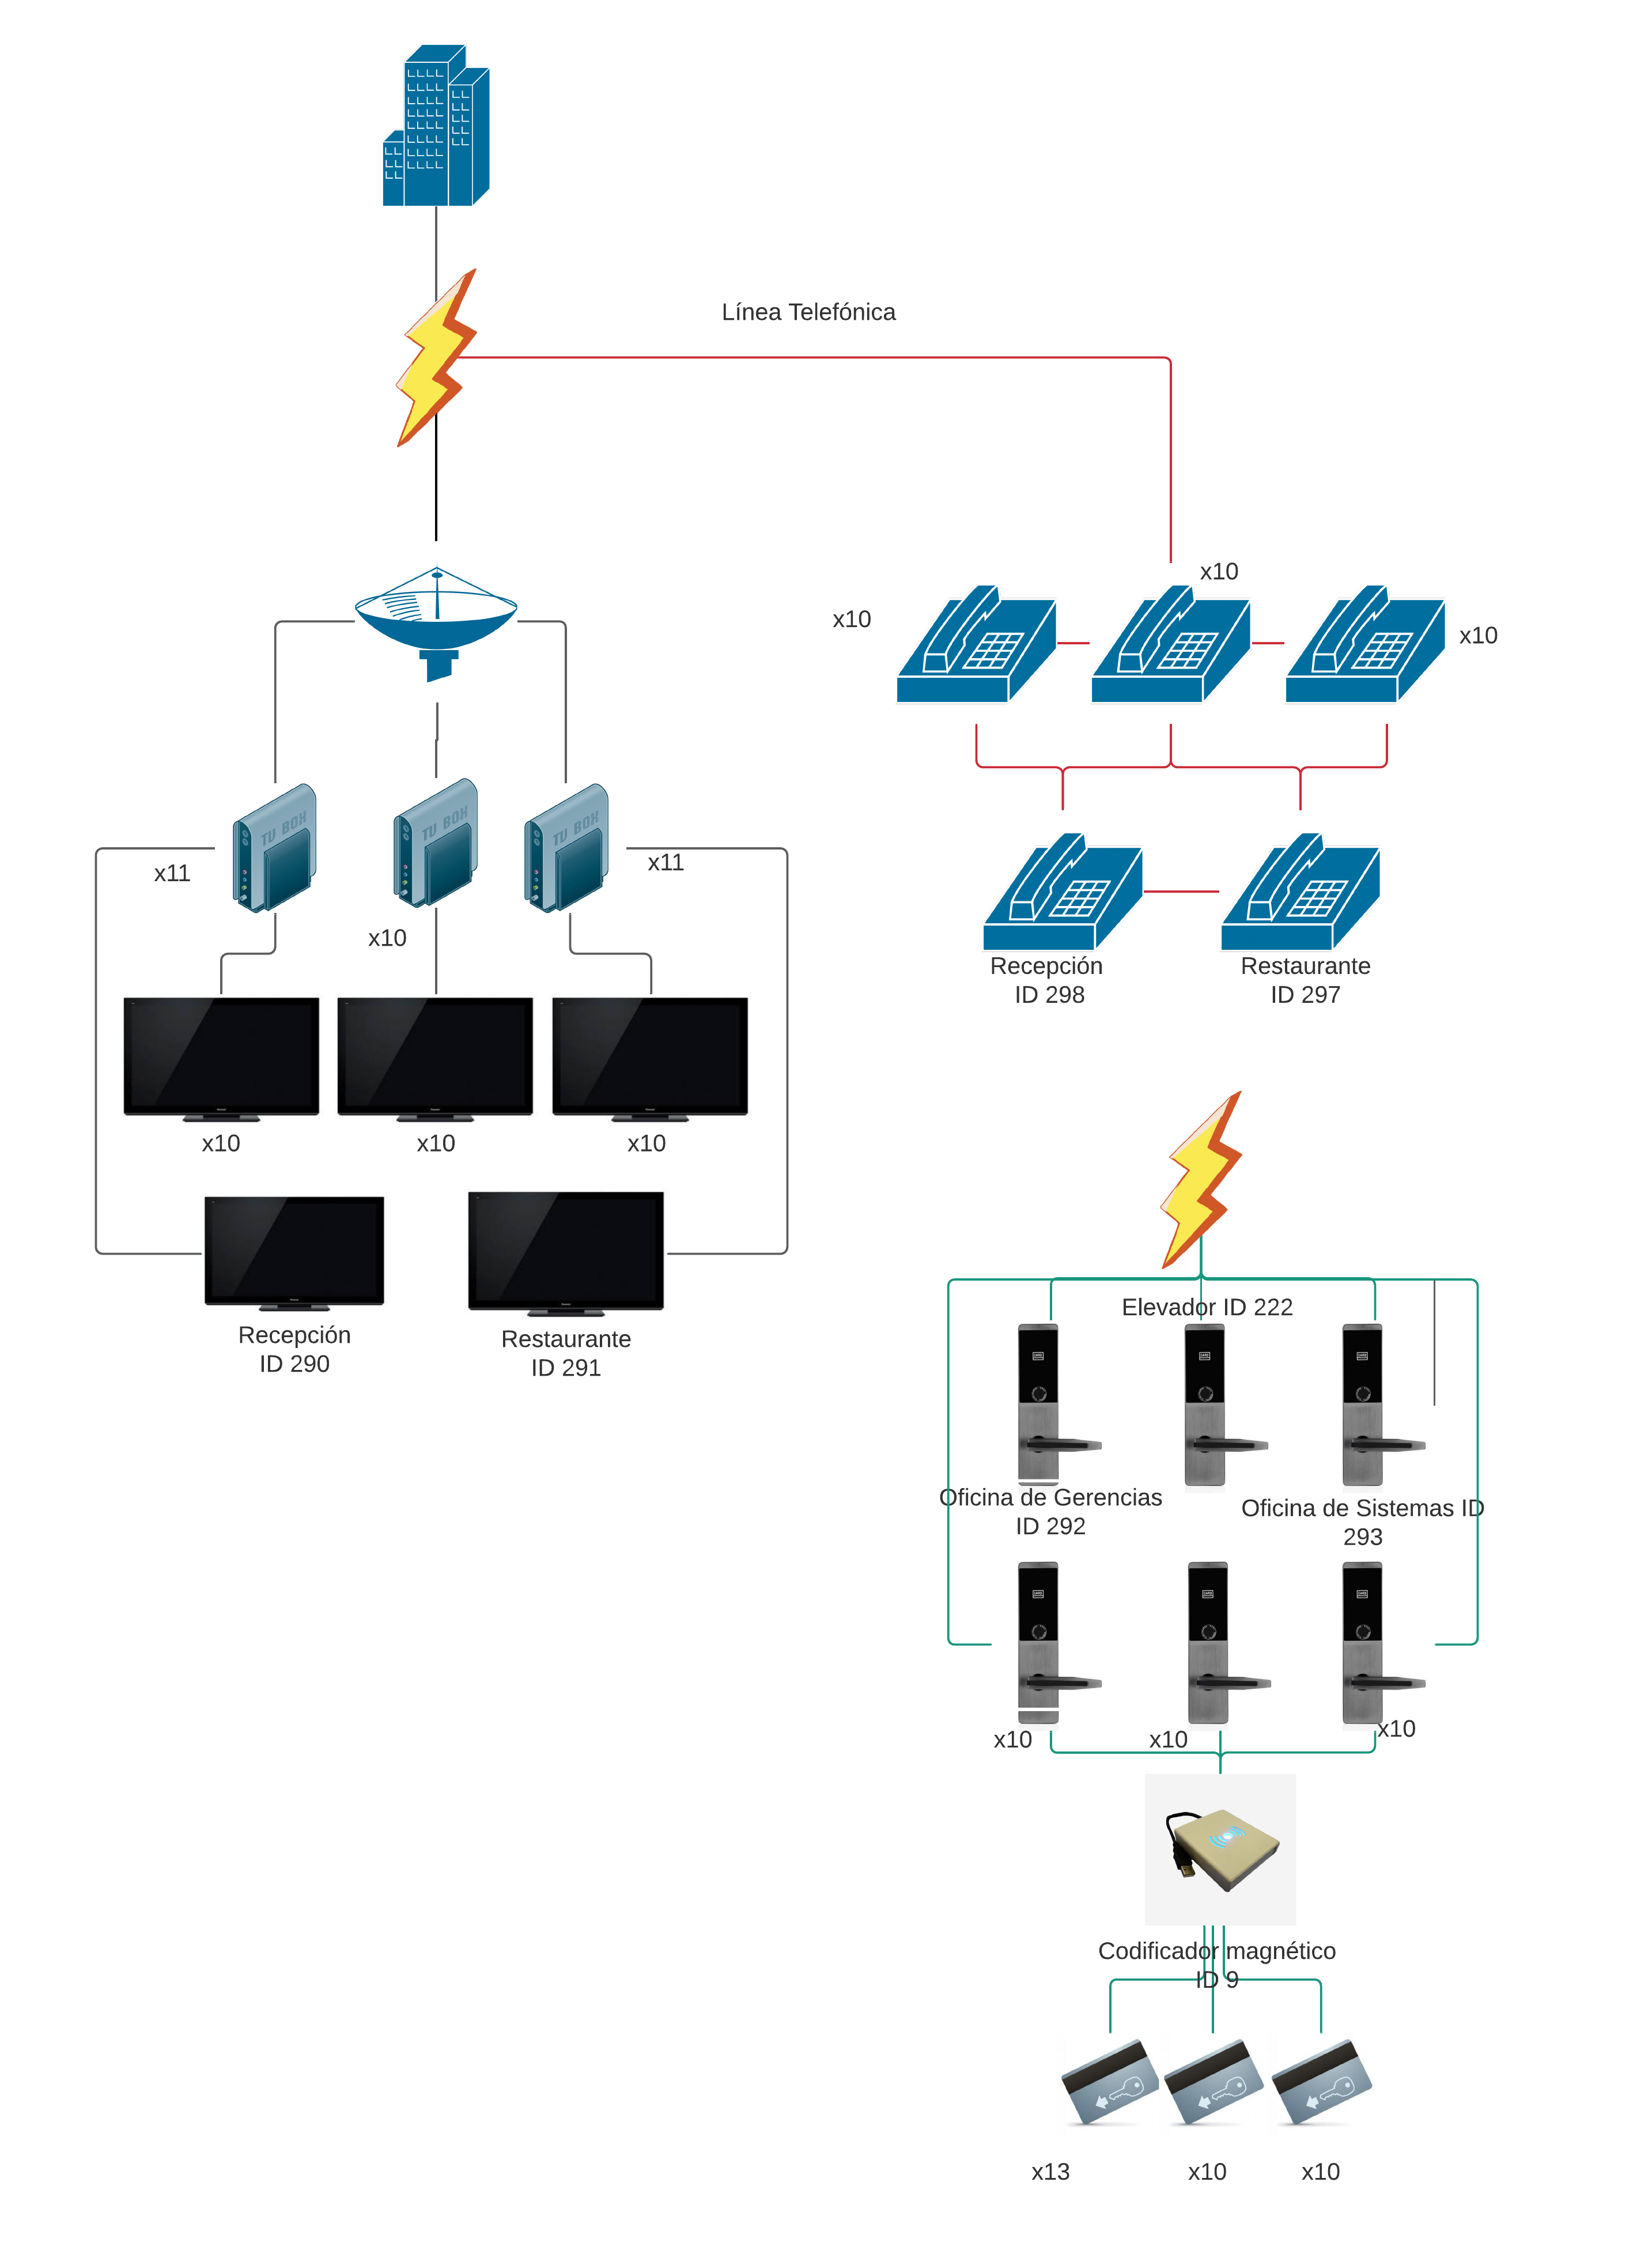
\includegraphics[width=\textwidth,height=\textheight,keepaspectratio]{imagenes/Diagrama 2.1.png}
    \caption{Diagrama otros activos}
    \label{fig:otros}
\end{figure}

En la figura \ref{fig:otros} se encuentra otro diagrama de activos, pero que no dependen de la red local. En esta encontramos tres clasificaciones diferentes que depende únicamente de la red de electricidad del hotel: el sistema de cable para televisiones, la línea de teléfonos, y las cerraduras de los cuartos. Aquí se procuró indicar el número exacto de activos de cada tipo, con el número general de activos por cuarto y luego especificando los que pertenecen a algún cuarto administrativo del hotel. Se separaron en dos partes, ya que la primera son servicios del hotel primero con lo es el cable especificado en negro que tiene su antena y sus aparatos para los canales para que funcione la televisión, y luego con rojo el servicio de telefonía. En la segunda parte con verde está todo el proceso de las cerraduras magnéticas, que involucra las mismas con su codificador de llaves para el acceso. 


En la tabla \ref{table:tabla2} se presentan las problemáticas encontradas relacionadas a la red de la imagen 2. Estas problemáticas son únicamente dirigidas a los dispositivos mencionados que son todos conectados a alguna fuente de electricidad. Es posible que, como problemática exista el forcejeo de la cerraduras o la entrada por ruptura de estas, pero al no ser problemas del tipo electrónico no fueron incluidos en la tabla. 

\begin{table}[H]
\begin{adjustbox}{max width=\textwidth}

\begin{tabular}{|l|l|}
\hline
\multicolumn{1}{|c|}{\textbf{Problemática}} &
  \multicolumn{1}{c|}{\textbf{Prevención}} \\ \hline
Generación de una llave maestra RFID & \begin{tabular}[c]{@{}l@{}} Tener un control de las llaves que terminen de usar los \\ huéspedes.
 \end{tabular} \\ \hline
Hackeo de la línea telefónica & \begin{tabular}[c]{@{}l@{}}Mantener contacto con la compañía que proporciona \\ el servicio para detectar dispositivos ajenos o \\ escuchas ilegales \end{tabular} \\ \hline
Hackeo de las antenas de televisión & \begin{tabular}[c]{@{}l@{}}Mantener en revisión y en mantenimiento \\ constante las antenas y los sintonizadores.
 \end{tabular} \\ \hline
Manipulación del Software de Restaurante & \begin{tabular}[c]{@{}l@{}}Tener la computadora del restaurante con protección (antivirus) \\ y no permitir el uso a gente que no esté autorizada.
 \end{tabular} \\ \hline  
Hackeo a la página web & \begin{tabular}[c]{@{}l@{}}Mantener en revisión y mantenimiento la \\ página además de tenerla protegida con algún software antivirus.
 \end{tabular} \\ \hline   
Robo en habitaciones por parte del personal & \begin{tabular}[c]{@{}l@{}}Restringir acceso a habitaciones solo a personal de limpieza \\ y mantenimiento en horas de trabajo \end{tabular} \\ \hline
Acceso de clientes a pisos que no son los suyos & \begin{tabular}[c]{@{}l@{}}Instalación de lector RFID en elevadores para limitar acceso de clientes a \\ únicamente el piso de su cuarto y áreas comunes.\end{tabular} \\ \hline
\begin{tabular}[c]{@{}l@{}}Utilización de llaves de reservaciones antiguas \\ para entrar a los cuartos \end{tabular} & ID único de tarjetas de acceso por reservación. \\ \hline
\end{tabular}%
\label{table:tabla2}
\end{adjustbox}
\caption{Problemáticas y prevenciones preliminares en otros activos}

\end{table}

\pagebreak

\section{Etapa 3}

\subsection{Definición de las vulnerabilidades}

Existen diversos factores que permiten que actores, internos o externos, logren vulnerar sistemas de la empresa. Factores como malas configuraciones, errores, descuidos, pueden resultar en escenarios fatídicos como el robo de información sensible o perdida de bienes, es por esto que las instituciones necesitan contar con soluciones para cada posible falla.


Un hotel puede tener muchas vulnerabilidades que van desde lo técnico hasta la propia ingeniería social, las vulnerabilidades principales encontradas en este caso son: 

\begin{itemize}
    \item Bases de datos en texto plano.
    \item Robo de información por navegación web.
    \item Poco nivel de seguridad en sistemas a nivel local.
    \item Exposición a intrusos en redes. 
    \item Malware y virus.
    \item Exposición ante dispositivos externos conectándose al Router administrativo de forma inalámbrica.
    \item Ransomware bloqueando infraestructura entera del hotel.
    \item Exposición por factores de ingeniería social.
    \item Exposición de hardware externo en los diversos activos tecnológicos del hotel.
\end{itemize}

Es de vital importancia entender como la práctica de defensa de sistemas tecnológicos puede prevenir y mitigar catástrofes que podrían costar mucho a las empresas, sobre todo cuando estas son pequeñas y medianas, por lo que el siempre contar con un plan de acción es la base para un buen sistema seguro.

\subsection{Medidas}

\subsubsection{MySQL}

Es aún muy común el mantener información dentro de las bases de datos en forma de texto plano, esto quiere decir que la información presente en las  bases de datos no cuenta con un cifrado en particular por lo que es completamente legible para aquel que tenga acceso a esta base de datos. Es por eso que empresas como Microsoft o IBM han empleado una tecnología conocida como Transparent Data Encryption (TDE) que ofrece un cifrado de datos a nivel archivo, o lo que también es llamado como datos en reposo. Si bien no es capaz de encriptar datos en tránsito, esta tecnología funciona a través de una certificación y una clave maestra, permitiendo que aquel que sea capaz de llegar a obtener esta información simplemente no pueda leerla pues quedará ilegible. Esta tecnología se encuentra disponible como parte de SQL Server de Microsoft en versiones desde 2008 hasta 2019, lo que se conecta directamente con otra vulnerabilidad \cite{ref9}.

El manejar la información desde un servidor local no suele ser la opción más segura existiendo otros servicios por lo que parte del plan de mitigación es migrar a una solución de SQL que este ubicada en la nube, esto se hace para evitar la exposición de los activos internos de la empresa; si bien es cierto que se puede asegurar el servidor de manera física en el hotel, es muchísimo más seguro que los datos se encuentren en un data center de una empresa responsable y madura. Este plan debe implementarse con su debido sistema de acceso a las bases de datos solamente a el personal con las credenciales correspondientes, éstas serían un nombre de usuario y una contraseña bastante robusta que no contenga ninguna especie de patrón fácilmente descifrable. Como se vio con anterioridad este tipo de servicios cuentan con tecnología de cifrado, lo que vuelve ilegible la información presentada para aquel que no cuente con la clave maestra, así como también evita la exposición a riesgos físicos que sí existen teniendo el servidor en las propias instalaciones del hotel.\cite{ref8}

\subsubsection{Firewall}

Hoy en día internet es una de las herramientas tecnológicas más usadas en el mundo, por esto mismo es también dónde puede existir mayor riesgo en cuánto a robo de información se trata. Además es uno de los medios por el cual un servidor puede llegar a sufrir mayor cantidad de ataques, por lo que para llevar a cabo una protección de estos ataques se propone el uso de un Firewall de Aplicaciones Web (WAF). Este tiene como principal función realizar un análisis de paquetes de petición ya sean HTTP o HTTPS, así como los modelos de tráfico. El Firewall examina cada petición que se es realizada al servidor antes de que llegue al cliente, esto en pro de asegurarse de que dicha petición cumple con las reglas establecidas por la configuración del Firewall. Este puede ser implementado tanto en software, ya sea instalando una aplicación en el sistema operativo que consumiría recursos del servidor local, como en hardware integrando funcionalidades en una solución $"appliance"$ lo que minimizaría de forma considerable la latencia pero generaría un mantenimiento y almacenamiento de equipos físicos llegando a ser bastante costoso. Existen dos tipos de WAF: de lista negra que se encargan de proteger contra ataques que ya sean conocidos, mientras que los de lista blanca solo admiten un tráfico que haya sido autorizado con antelación. El caso idílico es lograr trabajar con un híbrido capaz de poner ambos tipos en práctica.\cite{ref7}

En red local suelen existir un sin fin de amenazas ya sea provenientes de forma interna como de forma externa por lo que se llevará a cabo la implementación de un Next Generation Firewall (NGFW). Este es un nuevo sistema de seguridad para redes dentro de un dispositivo hardware o bien en una versión basada en software capaz de detectar ataques sofisticados, esto a través de forzar políticas de seguridad a nivel de aplicación, a nivel de puertos y protocolos de comunicación.
Estos mantienen las características de un Firewall con estado, se habla de filtrado de paquetes, compatibilidad con IPsec y VPN SSL, funciones de mapeo de IP, y supervisión de red. Sin embargo también cuentan con capacidades de inspección de contenido más profundas, debido a que son capaces de identificar ataques y malware, y además de bloquearlos al momento. Este Firewall es sobre todo recomendado para llevar a cabo un control del contenido de la red local hacia internet. Se debe tomar en cuenta que los NGFW son capaces de llevar a cabo inspecciones de SSL, App Control, previsión de intrusiones, y provee una  visibilidad de toda la superficie del ataque e inclusive incluye rutas para futuras actualizaciones proporcionando flexibilidad para evolucionar a través del panorama de amenazas manteniendo la red segura.\cite{ref6}

\subsubsection{Protocolos}

Es muy común en empresas enfrentarse a amenazas capaces de afectar el funcionamiento de los sistemas, como pueden ser las redes de comunicaciones, es por eso que existen estrategias para que la seguridad de los sistemas prevalezca, hablamos particularmente de \emph{Intrusion Prevention System (IPS)} y de \emph{Intrusion Detection System (IDS)}. IDS permite ver que está sucediendo en la red en tiempo real, esto a través de la recopilación de información, reconoce modificaciones y automatiza patrones de búsqueda en paquetes de datos enviados a través de la red, sin embargo este sistema solo es capaz de detectar, no previene ni detiene ataques. Es aquí donde entra IPS este es capaz de proteger sistemas de ataques e intrusiones, realiza análisis de tiempo real para determinar si se está produciendo o se va a producir alguna especie de incidente, esto a través de patrones, anomalías e inclusive comportamientos de carácter sospechoso, permite lanzar alarmas, descartar paquetes y desconectar conexiones. Es común encontrar tanto a IPS como IDS en productos mixtos, por lo que suelen ir de la mano y ayudaría a la infraestructura del hotel obtener una capa más para prevenir y remediar ataques. \cite{ref5} 

\subsubsection{Antivirus}

Los virus de computadora son una de las problemáticas más frecuentes que existen en la actualidad, pudiendo llegar desde a dispositivos de uso domestico hasta dispositivos corporativos. Ante estas amenazas tan comunes se propone la implementación de un antivirus, estos tienen la misión principal de detectar y eliminar todo software malicioso de equipos y dispositivos. Realizan análisis continuos los cuales hacen una comparación de archivos presentes en el sistema operativo contra una base de datos que contiene firmas, las cuales son características identificativas de diversos tipos de malware, esta bases de datos están en continua actualización. Algunos antivirus son capaces de detectar diversas amenazas mediante la identificación de patrones en archivos localizando alteraciones del sistema o analizando comportamiento que no suelen ser normales en algunos componentes informáticos. Protegen de amenazas como virus, los cuales son programas maliciosos que se esconden como ficheros de usuario con el propósito de acceder a equipos sin consentimiento, y tienden a robar información, borrar archivos o alterar configuraciones del equipo.
Existen los gusanos informáticos los cuales son programas diseñados para ejecutarse y propagarse a través de una red con el objetivo de colapsar equipos y redes. \cite{ref4}

En ocasiones existen vulnerabilidades tan obvias como dispositivos externos a la institución conectándose a la red administrativa sin autorización, por lo que el protocolo recomendado para evitar este tipo de filtraciones es WPA2 el cual mejoró a la versión anterior es decir WEB, implementando dos nuevos protocolos como lo son negociación de 4 mensajes y negociación de clave de grupo, esto permite establecer y cambiar de forma apropiada las claves criptográficas. \cite{ref3}

El antivirus cotizado para ser implementado en los dispositivos del hotel es la licencia de Kaspersky específicamente ``Internet Security'' se recomienda contratar el plan anual para 5 dispositivos a un precio de 1,119 MXN y un plan anual para 3 dispositivos a 979 MXN, cabe destacar que si bien se contrata las licencias para un total de 8 dispositivos, el hotel solo cuenta con 7 sin embargo esto se decide así debido a que contratar un plan para 3 dispositivos es más barato que dos planes individuales los cuales tienen un costo anual de 559 MXN. \cite{ref13}

\subsubsection{Copias de Seguridad}
El Ransomware es un software de carácter extorsivo de modo que la finalidad que tiene es impedir el uso de un dispositivo hasta que no se haya pagado un rescate, la forma en la que se lleva a cabo es introduciéndose al dispositivo y cifrando parte o todo el sistema operativo, para prevenir ataques de este tipo es fundamental mantener todos los dispositivos actualizados y llevar a cabo un uso responsable del dispositivo \cite{ref1}.

Por otro lado en caso de tener un ataque de Ransomware en el cual detenga operaciones completas se recomienda que el hotel posea una copia de seguridad en frío o también conocida como fuera de línea, es una copia de seguridad de la infraestructura entera que no se accederá con frecuencia, pero si se actualiza con frecuencia. Es la forma más segura de realizar copias de seguridad debido a que evita el riesgo de copiar datos que puedan estar en un proceso de actualización, sin embargo esta implica tener un tiempo de inactividad por lo que los usuarios no pueden acceder a los activos involucrados. Debido a que se tiene inactividad al hacer esto, se recomienda hacer estos respaldos a altas horas de la noche cuando el uso de los aparatos es muy bajo, y para el caso de los equipos de recepción estos no deben respaldarse al mismo tiempo. Además de contarse con un respaldo en site que a diferencia del anterior que era un respaldo completo, este simplemente sería un respaldo incremental la cual solo agrega información cuando se agrega al equipo, mientras que si es completo este hace un respaldo de maquina entera. Un ataque de Ransomware puede suceder en cualquier momento por lo que como respuesta a este tipo e incidentes por lo que se tiene una imagen de cada computadora con programas mínimos que permitan el funcionamiento correcto de la empresa en lo que son recuperados dichos respaldos \cite{ref2}. 

\subsubsection{Protección del Hardware}

Las empresas tienen una gran vulnerabilidad a la cual no suele ponerse atención sin embargo es una debilidad con el potencial de ser más devastadora que el apartado técnico y se trata de ingeniería social, la cuál es la práctica de obtener información, accesos o permisos a través de manipular usuarios legítimos, esta clase de problemas necesita sobre todo un programa de entrenamiento en el cual se lleve a cabo una capacitación de todo el personal acerca de medidas que deben tomarse para evitar riesgos en los activos tecnológicos de la empresa, este programa debe ser personalizada y centrada en función de las necesidades específicas, debe ser periódico y ser actualizado durante el tiempo \cite{ref11}, las medidas que deben emplearse son:
\begin{itemize}
    \item Prohibición de acceso a áreas no autorizadas, el personal del hotel debe mantenerse alejado de aquellas áreas que no le competen, sobre todo en áreas que puedan poner en riesgo los activos T.I. de la empresa.
    \item Especificar el uso en todo momento de una identificación en la que se muestre nombre, área de trabajo y puesto, para evitar que personas ajenas al hotel finjan ser empleados del mismo.
    \item El personal no puede tener acceso a información que no le corresponde dígase bases de datos, configuraciones de red, por lo que se limitarán las credenciales de acceso única y exclusivamente a las personas que les corresponda.
    \item Informar y capacitar empleados acerca de las amenazas más comunes en ciberseguridad como phishing o malware.
    \item Toda cuenta del personal debe estar asegurada con método de doble autenticación.
    \item Principio de mínimo privilegio, el cual consiste en la configuración de cuentas para que estas no dispongan de privilegios de administrador y reduciendo las acciones que se puedan realizar en estos a lo mínimo para que puedan llevar a cabo su trabajo.
    \item Sin embargo hay una amenaza que no suele tomarse en cuenta que es un ataque a consciencia del propio personal, por lo que se llevará a cabo la instalación de un write blocker físico, dispositivo capaz de interceptar cualquier escritura de disco inadvertida, al detectar actividad maliciosa se detendrán las operaciones en dicho dispositivo, se instalará el dispositivo por protocolo, se copia el disco duro y se lleva a cabo una auditoría desde el disco copiado, esto se realiza para conservar la integridad en la evidencia y el empleado no pueda alegar que se haya agregado información con el fin de inculparlo, write blocker no puede quedarse instalado de forma permanente en el dispositivo pues la computadora dejaría de funcionar.
    \item Se prohíbe el acceso con cualquier herramienta en la que se pueda capturar información, esto puede ser desde un celular hasta cualquier tipo de papel, esto permite evitar cualquier robo de información por medios externos de la empresa.
    
\end{itemize}

En cuanto a la seguridad del hardware en físico existen muchos elementos que hay que plantear para su protección. El primer punto estaría en el lugar del hotel en el que estén localizados los servidores, ya que debe de ser un lugar alejado del acceso al personal no autorizado. Es muy probable que no todas las edificaciones se hayan planeado con la intención de tener un cuarto seguro para almacenar la información, pero se pueden tomar medidas que ayuden a contra restar esto. En lo que respecta a la seguridad del cuarto en sí, se deben de tener planes contra elementos que comprometan la integridad de los servidores, como lo podrían ser incendios, filtraciones de agua, o externos que pretendan dañar el sistema. Claro que la opción más segura sería la reestructuración de este cuarto para que estos no sean problemas sea la mejor opción, pero también sería algo bastante costoso que no sería viable en principio para una PyME. Es por ello que soluciones alternativas en este caso serían lo mejor, como la instalación de sistemas contra incendios, capacitación al personal en el caso de desastres, copias de seguridad en frío como se habían mencionado anteriormente, y pólizas de seguro para proteger a este equipo.   

Y como segundo punto estaría en lo que respecta a la seguridad de este hardware para robo de información en físico. Es importante mantener los equipos seguros en la parte del costo que representaría si se daña, pero es aún más el costo que tendría el robo de información por la posible pérdida de confianza de los clientes o de la productividad en lo que se regresa a la actividad normal. Es por ello que como se mencionó anteriormente, debe de haber un control del personal que no sea necesario en este ámbito, además de huéspedes que puedan llegar. Las personas responsables deben de realizar constantes revisiones al sistema en búsqueda de dispositivos externos que se dediquen a robar la información de manera remota, y asegurarse que no tengan conectados nada inusual. También estaría la opción de desactivar todos los puertos que no se encuentren en uso, ya que de lo contrario son susceptibles a estos accesos no deseados. Estas acciones son posibles de llevar a cabo con una simple planeación, y no ocupan de muchos recursos económicos del hotel. 

\subsubsection{Reportes Post Mortem}

Cada que ocurra un incidente se debe realizar un reporte post mortem en el que se detalle lo siguiente: 

\begin{itemize}
    \item Suceso.
    \item Involucrados.
    \item Activos afectados.
    \item Respuesta.
    \item Downtime (hubo o no hubo y en caso de que sí, cuanto).
    \item Perdidas.
    \item Oportunidades detectadas.
    \item Que acciones fueron implementadas de forma correcta.
\end{itemize}

Esto para poder ser un proceso de mejora continua.

 Para que este plan sea un programa de seguridad integral y completo, el propósito se basó en cumplir de forma adecuada con el pilar fundamental de la ciberseguridad el cual es la tríada CIA, Confidentiality, Integrity And Availability (confidencialidad, integridad y disponibilidad). 
 El modelo presentado es Zero Trust por lo que se asume que puede haber atacantes tanto dentro de la red como fuera de ella, por lo que no se debe confiar en ningún usuario o dispositivo de forma predeterminada.

\subsection{Costos del Plan de Mitigación}
\subsubsection{Cotización Azure}
Este plan de mitigación hace 1 década o 5 años hubiera forzado a PyME's a tener que encontrar servicios por todos lados en constantes llamadas para poder asegurar que la mayoría de su red no pueda ser robada. Dado el crecimiento que se ha tenido en la tecnología, ya existen empresas de confianza como Amazon Web Services, Microsoft Azure, u Oracle que te pueden hacer un paquete de servicios necesarios para la seguridad de tu empresa y te facilita todos los aspectos. En vez de tener que andar en constante busca por servicios por el internet en Microsoft por ejemplo te vas a la calculadora de precios e ingresas los servicios necesarios. En este caso necesitamos lo siguiente: Transparent Data Encryption (TDE), Microsoft SQL server, Firewall, Intrusion Prevention System (IPS), Intrusion Detection System, antivirus, y Ransomware.  


Luego incluyendo todos los demás servicios de Azure que en este caso serian Azure database for MySQL, Azure Firewall, Azure Backup, y Azure Defender. Estos servicios son los que podrían cubrir todo lo necesario en este caso para tener una seguridad impecable en el hotel. El costo mensual seria alrededor de los 908 USD, pero no solo cubriría ese tipo de situaciones, sino hay varios servicios de Azure que podrían hacer un servicio superior a lo que necesitas para poder garantizar de manera superior un nivel de seguridad. Estas medidas con Azure si se conecta de manera apropiada podrían servir a la empresa de manera inmediata para que desde el día 1 ya tengan la seguridad que necesitan para proteger su negocio. Debido a el numero de oferta que ha tenido el crear servicios de seguridad en el internet y todo relacionado con la nube, existe una gran posibilidad de que por temas de economía pueda reducir su costo aunque la demanda siga subiendo pero cada día existen más empresas tratando de ofrecer servicios debido al margen alto que están recibiendo los grandes como Amazon y Microsoft \cite{ref10}. 



\subsubsection{Cotización AWS}

Otra alternativa recomendada para el uso del hotel es la de Amazon Web Services que maneja esquemas de precios mucho más adecuados a una PyME. 

El primer servicio que debe considerarse es AWS RDS que es una base de datos conectada con MySQL y el AWS Shield Standard que incluye protección contra ataques DDoS comunes. El costo de este plan es de 12.41 USD mensuales e incluye el Shield Standard sin costo adicional. Otro de los paquetes de servicios recomendados para la empresa es la utilización de instancias AWS EC2 para migrar el hosting de la página web a la nube de Amazon y asegurarla con ellos, el AWS CloudTrail que es un sistema de registros para eventos de AWS, este permitirá auditar la actividad que los empleados realicen con los activos de AWS, el AWS KMS que es un administrador de claves y uso de cifrado de Amazon enfocado en seguridad de hardware, el AWS S3 Glacier que es el sistema de copia de seguridad en frío. Todos estos servicios por un precio total de 91.55 USD mensuales, y para el caso de las instancias de EC2 si fuese necesario se pueden pedir más recursos bajo demanda si se llegase a tener una temporada muy ocupada. Estos precios son mucho mas reducidos en comparación con Azure, sin embargo no se están ofreciendo los mismos servicios en ambos pero AWS tiene la ventaja de manejar mensualidades por volumen para dar el costo final \cite{ref12}.

La cotización se puede consultar en:\\
%favor de no modificar nada, este link es permanente
\url{https://calculator.aws/#/estimate?id=288c678905b84da7bf504a7ea262b5e6a0afc4c7}


Como resumen de esta etapa podemos ver el diagrama final de nuestra red (Figura \ref{fig:diag_final}) con las estrategias de mitigación añadidas y una tabla de estas mismas (Tabla \ref{tab:pt1}).

\begin{figure}[H]
    \centering
    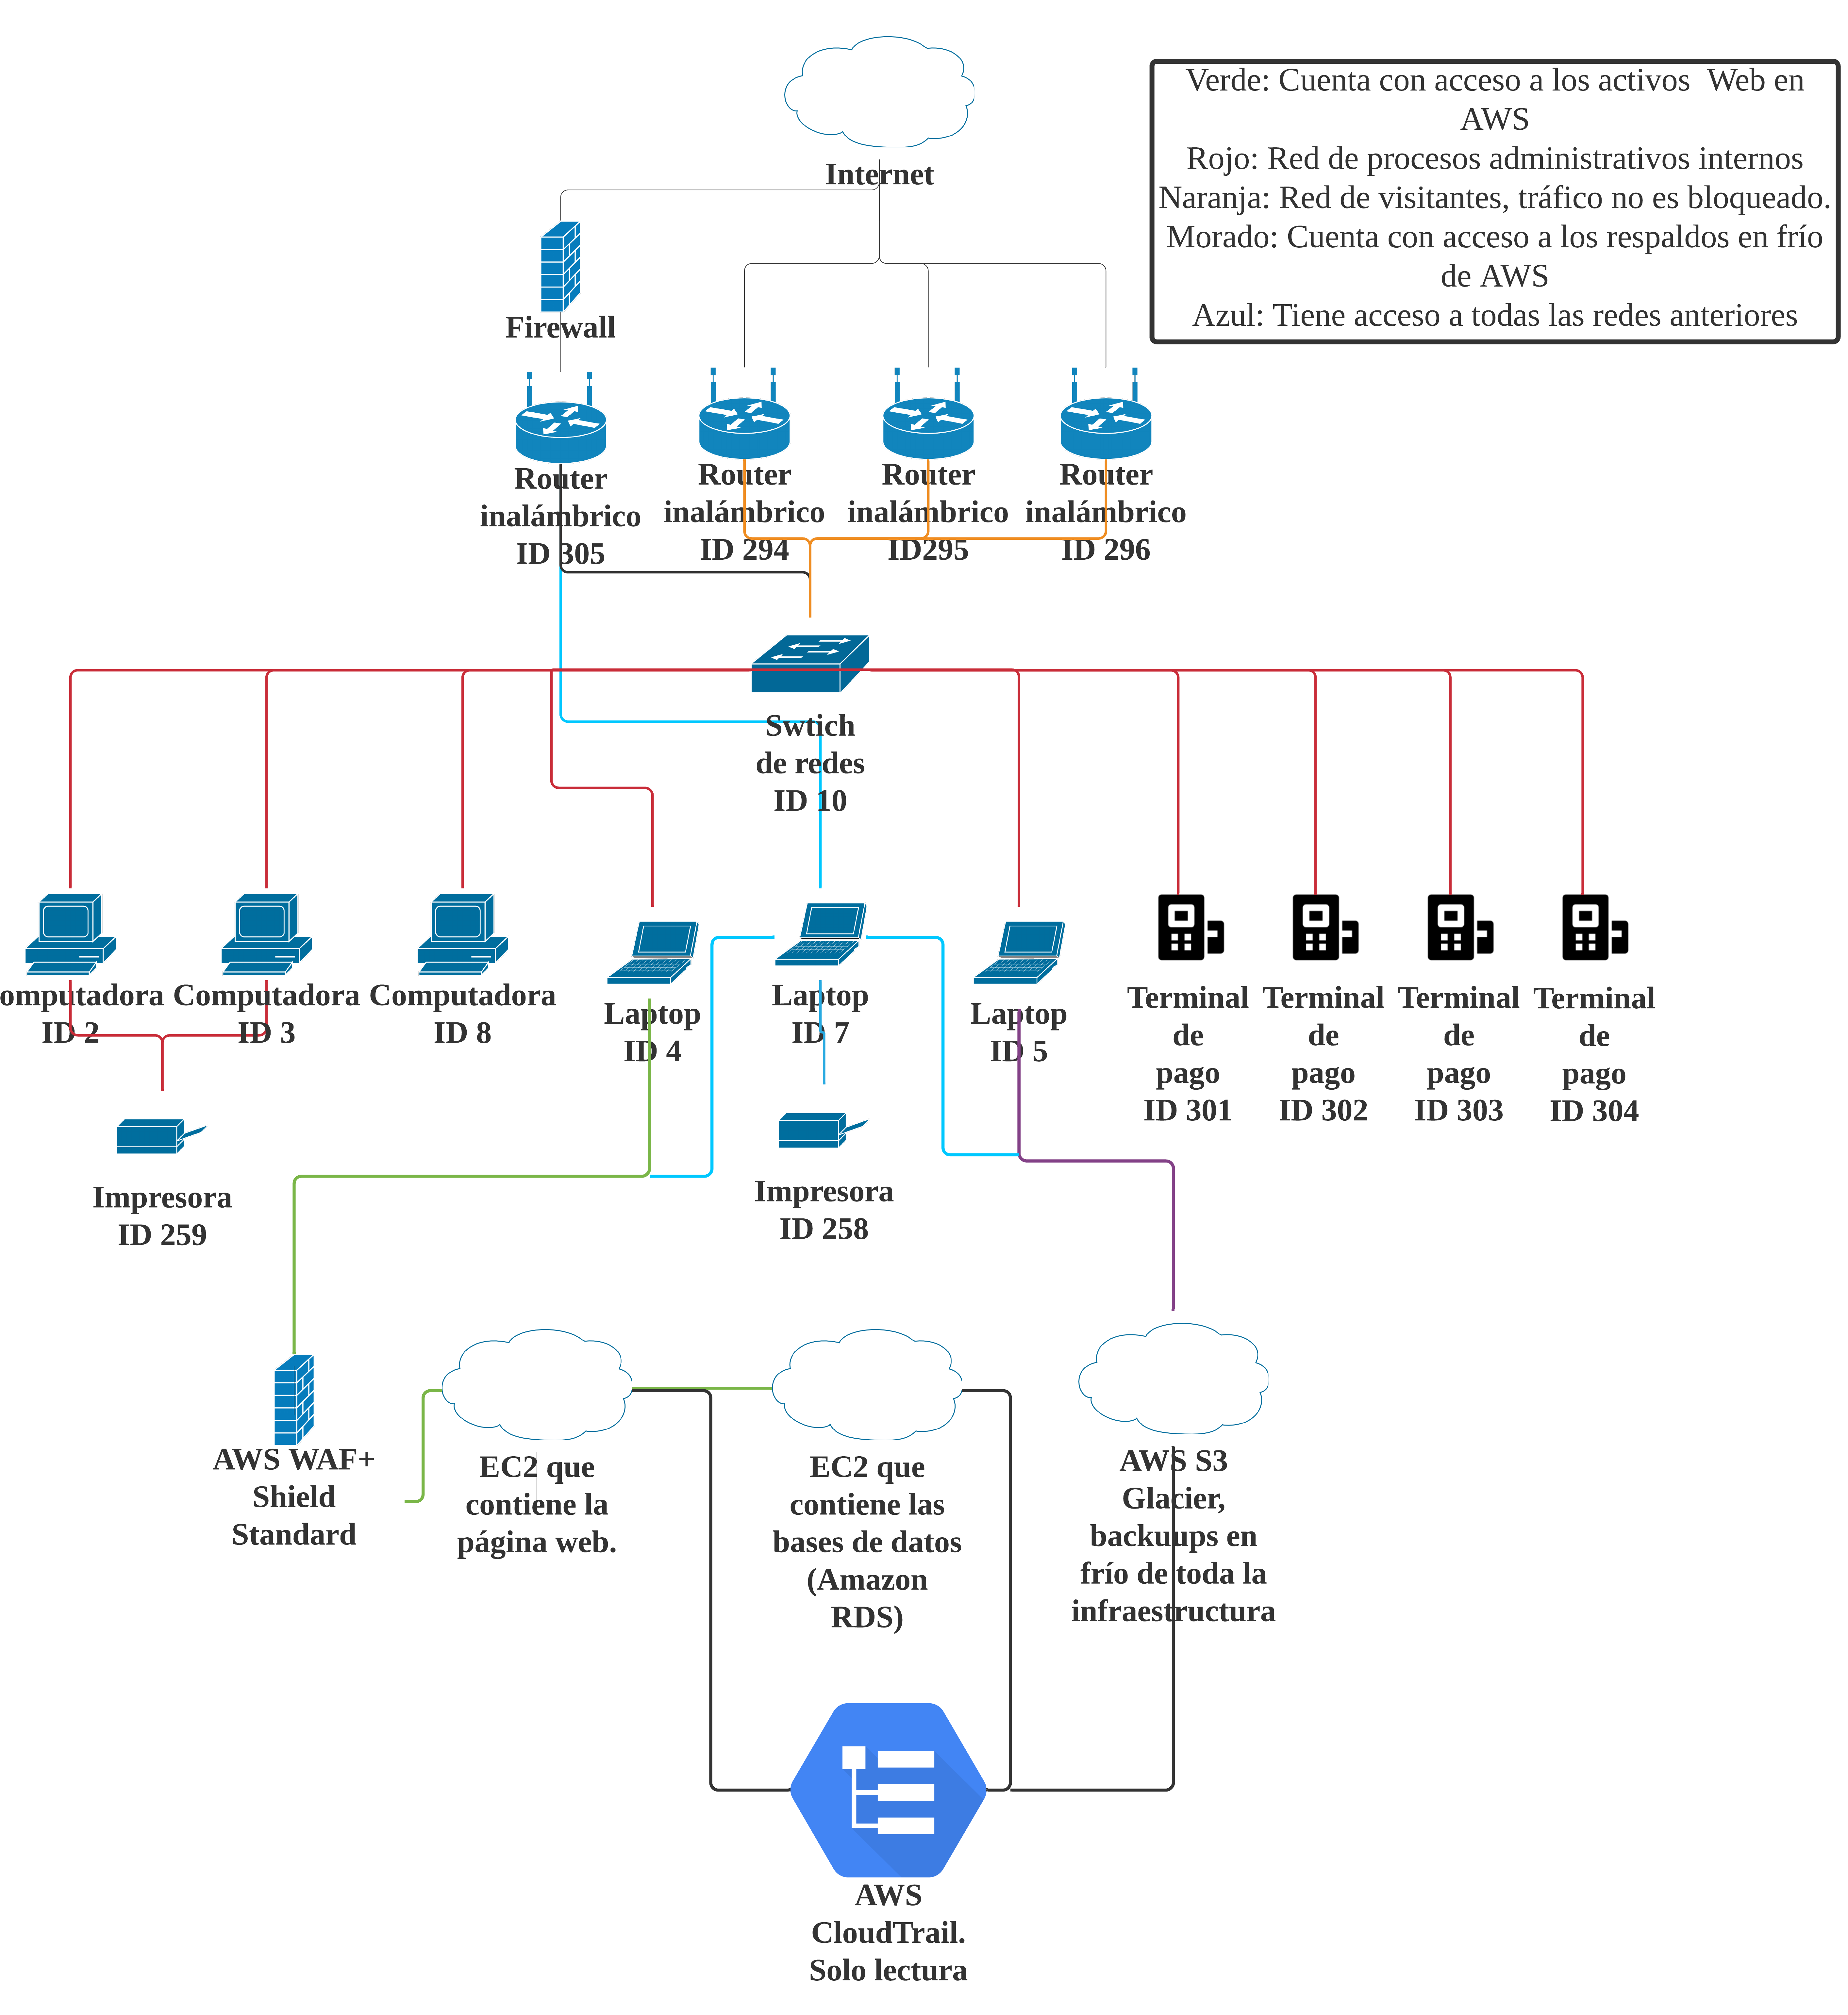
\includegraphics[width=1\textwidth]{imagenes/Diagrama_Final.png}
    \caption{Diagrama de red final.}
    \label{fig:diag_final}
\end{figure}

\clearpage

\begin{table}[H]
\begin{adjustbox}{max width=\textwidth}
\begin{tabular}{|l|l|l|}
\hline
\# de estrategia &
  Nombre &
  Descripción \\ \hline
1 &
  Áreas restringidas &
  \begin{tabular}[c]{@{}l@{}}El personal del hotel debe mantenerse alejado de\\  aquellas áreas que no le competen, sobre todo en\\ áreas que puedan poner en riesgo los activos T.I. \\ de la empresa.\end{tabular} \\ \hline
2 &
  Uso de identificación &
  \begin{tabular}[c]{@{}l@{}}Especificar el uso en todo momento de una\\  identificación en la que se muestre nombre, área \\ de  trabajo y puesto, para evitar que personas\\ ajenas al hotel finjan ser empleados del mismo.\end{tabular} \\ \hline
3 &
  Acceso a información restringido &
  \begin{tabular}[c]{@{}l@{}}El personal no puede tener acceso a información\\ que no le corresponde dígase bases de datos, \\ configuraciones de red, por lo que se limitarán las\\ credenciales de acceso  única y exclusivamente \\ a las personas que les corresponda.\end{tabular} \\ \hline
4 &
  Capacitación a empleados &
  \begin{tabular}[c]{@{}l@{}}Informar y capacitar empleados acerca de las \\ amenazas más comunes en ciberseguridad \\ como phishing o malware.\end{tabular} \\ \hline
5 &
  Doble autenticación &
  \begin{tabular}[c]{@{}l@{}}Toda cuenta del personal debe estar asegurada\\ con método de doble autenticación.\end{tabular} \\ \hline
6 &
  Principio de mínimo privilegio &
  \begin{tabular}[c]{@{}l@{}}Consiste en la configuración de cuentas para \\ que estas no dispongan de privilegios de\\ administrador y reduciendo las acciones que\\ se puedan realizar en estos a lo mínimo para \\ que puedan llevar a cabo su trabajo.\end{tabular} \\ \hline
%\caption{Tabla de estrategias parte 1.}
%\label{tab:pt1}
\end{tabular}%
\end{adjustbox}
\end{table}


\begin{table}[H]

\begin{adjustbox}{max width=\textwidth}
\begin{tabular}{|l|l|l|}
\hline
\# de estrategia &
  Nombre &
  Descripción \\ \hline
7 &
  Write Blocker &
  \begin{tabular}[c]{@{}l@{}} En caso de detectar actividad maliciosa  en un equipo,\\ se detendrán las operaciones en dicho dispositivo, \\se usará el Write Locker para copiar el disco duro \\ y se lleva a cabo la auditoría desde el disco copiado.\\ Esto se realiza para conservar la integridad de la \\ evidencia y que el empleado no pueda alegar que \\ se ha agregado información al disco con el fin de \\ inculparlo.\end{tabular} \\ \hline
8 &
  Herramientas de captura prohibidas &
  \begin{tabular}[c]{@{}l@{}}Se prohíbe el acceso con cualquier herramienta \\ en la que se pueda capturar información, esto \\ puede ser desde un celular hasta cualquier tipo \\ de papel, esto permite evitar cualquier robo de \\ información por medios externos de la\\ empresa.  \end{tabular} \\ \hline  
\end{tabular}%
\end{adjustbox}
\label{tab:pt1}
\end{table}

\subsection{Costo final del plan de mitigación}

Al escogerse el plan anual de Amazon Web Services y los planes de antivirus de Kaspersky el total anual del plan de mitigacion es de 23,761.46 MXN al año.


\section{Etapa 4. Discusión, conclusiones y evaluación final.}

\subsection{Técnicas y herramientas de ingeniería empleadas}

Técnicas de ingeniería empleadas:
\begin{enumerate}
    \item Levantamiento de inventario de activos
    \item Registro de empleados 
    \item Registro de ubicaciones de la empresa
    \item Mapeo de redes de activos 
    \item Análisis de vulnerabilidades
    \item Compromiso ciudadano para la transformación social
    \item Argumentación ética
    \item Seguridad informática
    \item Algoritmos criptográficos
    \item Principio de mínimo privilegio
    \item Control 17
\end{enumerate}
Herramientas de ingeniería empleadas:
\begin{enumerate}
    \item MySQL
    \item phpMyAdmin
    \item Calculadora de precios de Amazon Web Services
    \item Calculadora de precios de Microsoft Azure 
\end{enumerate}

\subsection{Infraestructura}

Para llevar a cabo el proyecto es necesaria la siguiente infraestructura:
Servicios virtualizados de Amazon Web Services: 
\begin{enumerate}
    \item Servicio AWS Cloud Trail
    \item AWS Key Management Service
    \item AWS Web Application Firewall (WAF)
    \item 2 instancias de Amazon EC2 t3 micro de 30 GB de almacenamiento 
    \item Amazon Simple Storage Service (S3) 2TB
    \item Amazon RDS for SQL server db.t2.micro de 30 GB con 2 nodos 
\end{enumerate}

También se requiere capacitar a los empleados del hotel sobre amenazas comunes en ciberseguridad, y un write blocker en caso de requerir auditar un equipo. Además, en caso de que el hotel no contase con las licencias de Windows 10 pro, se deben adquirir pues son necesarias para poder aplicar el principio de mínimo privilegio. 

\subsection{Conclusiones}

En conclusión el plan de mitigación se diseño con éxito y es capaz de brindar la cobertura deseada a un precio razonable para una PyME, con un costo que justifica la inversión y permite tener respaldos en caso de que suceda un desastre y se tenga que restaurar una versión anterior de los sistemas. El plan es escalable y afín a empresas de giro similar, por lo que su diseño es sólido. El uso de sistemas virtualizados agrega una capa de seguridad extra pues la responsabilidad de la empresa contratada el cuidar que no existan accesos no autorizados a los equipos que mantienen estos recursos. 



\newpage

\bibliographystyle{ieeetr}
\bibliography{referencias.bib}

\end{document}
